\documentclass[12pt]{book}
\usepackage{graphicx}
\usepackage{mathtools}
\usepackage{xcolor}
\usepackage{enumitem}
\parindent 0pt
\parskip 6pt
\begin{document}
\title{
piHPSDR User's Manual
}
\author{
Christoph van W\"ullen, DL1YCF
}
%
\maketitle
\tableofcontents
\chapter{Introduction}
piHPSDR is a program that can operate with software defined radios (SDRs). As a graphical user interface,
it uses the GTK-3 toolkit, while the actual signal processing is done by Warren Pratt's WDSP library. Thus,
piHPSDR organizes the transfer of digitized radio frequency (RF) data between the radio hardware and the WDSP library, the
transfer of audio data (either from a microphone or to a headphone), as well as the processing of user
input (either by mouse/touch-screen, keyboard, or external "knobs and buttons"),
 and the graphical display of the RF data. piHPSDR is intended
to run on different variants of Unix. It runs on all sorts of Linux systems, including a Raspberry Pi (hence
the name piHPSDR), but equally well on Linux desktop or laptop computers, and on Apple Macintosh (Mac OSX)
computers which have a Unix variant under the hood. The present author is not aware of piHPSDR running
under the Windows operating system, although with environments such as MinGW, this should be possible.

Although piHPSDR can be operated entirely by using mouse and keyboard as input devices, many users prefer to
have physical push-buttons and/or knobs or dials. To this end, piHPSDR can control push-buttons and rotary
encoders connected to the GPIO (general purpose input/output)
lines of a Raspberry Pi. At least two generations of such controllers have
been put on the market by Apache labs, and I know of several projects where home-brewn controllers have
successfully been made. As an alternative, MIDI devices can be used for user interaction. For desktop/laptop
computers that do not have GPIO lines, MIDI offers an easy-to-use possibility of having push-bottons and
dials that control piHPSDR. Apart from homebrew projects in which a micro-controller such as an Arduino Micro
controls the actual buttons/knobs and acts as a MIDI device to the computer to which it is connected via USB,
there are low-cost so-called "DJ controllers" (DJ stands for disk jockey) from various brands which have
successfully been used with piHPSDR. A third possibility to control piHPSDR is via a serial interface
through CAT (computer aided transceiver) commands. The CAT model used by piHPSDR is based on the Kenwood
TS-2000 command set with lots of PowerSDR extensions.

Using a touch-screen instead of a mouse offers the possiblity to put the actual radio hardware together
with a Raspberry Pi running piHPSDR and an assortment of buttons/knobs into a single enclosure. This way,
one can build an SDR radio which can be operated like a conventional analog one.

The piHPSDR program has been written by John Melton G0ORX/N6LYT. It is free software that is licensed under
the GNU (free software foundation) general public license. Many other radio amateurs have contributed to
the code. A lot of extensions and improvements have been added by myself, therefore this document refers
to the version of piHPSDR that can be found on my github account \texttt{https://github.com/dl1ycf/pihpsdr}.

Because piHPSDR can be used on many different types of computers, and because operating systems change
rather quickly over time, I generally do not recommend to have a ,,binary release'' with files that you
can just copy to your computer and then it runs. Instead, my personal recommendation is to build piHPSDR
and WDSP from the sources, only this procedure guarantees compatibility of the final program with your
operating system. A manual of how to compile piHPSDR from the sources is available separately,
see \texttt{https://github.com/dl1ycf/pihpsdr-compile-from-sources}, so this will not be covered in 
the present manual. This manual starts with the first invocation of a freshly compiled piHPSDR.

\chapter{Starting piHPSDR for the first time}
Let us assume you have an SDR (say, an ANAN-7000 or a HermesLite-II) powered up and connected to an antenna,
and you have piHPSDR installed on a computer (say, a Raspberry Pi or an Apple Macintosh), the first thing to
do is to establish a proper connection between the computer and the radio. Although advocated at many places,
I do highly recommend against a WiFi connection. WiFi routers often use ,,optimizations'' where they hold
back data packets for a given client for a while, to be able to send a collection of them in a burst. While
this certainly optimizes the through-put because it minimizes clear-channel arbritration events, such jitters
are desastrous in SDR operation. The safest way of connecting the radio and the computer is to have a
managed switch with a built-in DHCP server, and to connect both the computer and the radio with a suitable
cable to the switch. If the computer has both a RJ45 jack for an ethernet cable, and a WiFi interface, my
personal recommendation is to use WiFi to connect to the internet, and use a single ,,direct cable'' plugged
into the RJ45 jacks of the computer and of the radio. This is a little bit tricky since both the computer
and the radio have to be set to a fixed IP address (e.g. computer: 192.168.1.50, radio: 192.168.1.51) with
the same netmask. However, once this has been done, this is the safest connection with no perturbations from
elsewhere.

\newpage
If the piHPSDR program is started for the first time, it opens a window that looks like this

\begin{center}
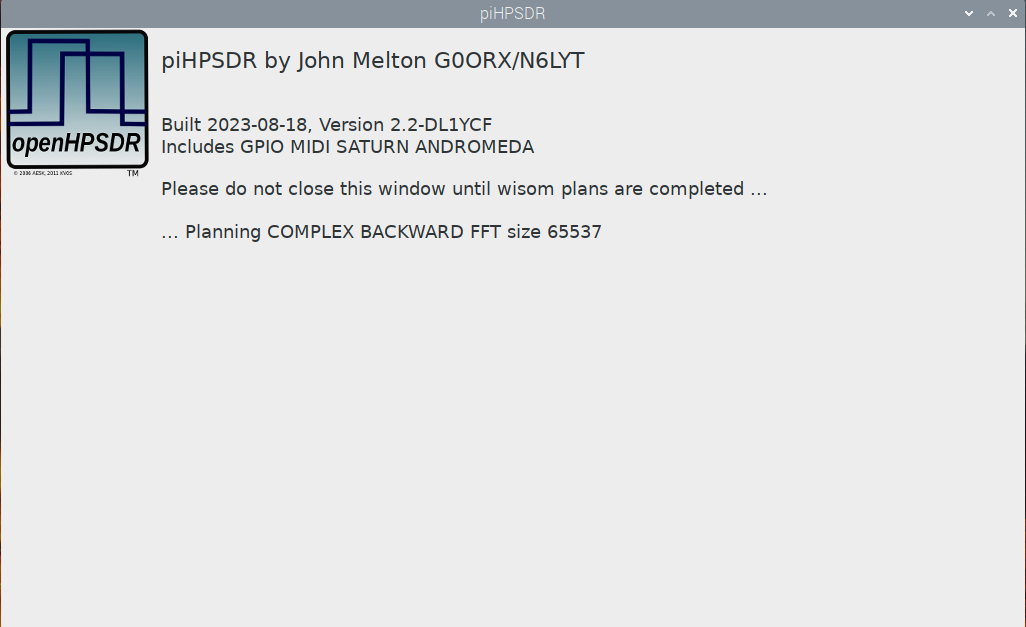
\includegraphics[width=12cm]{Planning.png}
\end{center}

besides stating a version number and when piHPSDR was built, a list of optional features (to be activated
at compile time) is stated, in this case, GPIO, MIDI, SATURN, and ANDROMEDA. These options indicate
that the program has GPIO support (this is only possible on Raspberry Pi or similar single board computers),
that is has support for MIDI devices, that it can run natively on the compute module of the latest
G2 (generation two) SDRs from Apache labs, and that is has support for Laurence Barker's ANDROMEDA controller.
What is important here that you have to wait. This only applies to the very first time you start piHPSDR.
On CPUs with a rather simple instruction set (like the ARM processor in the Raspberry Pi, or the Apple
Silicon processor in recent Macintosh computers), this "planning" step is quite fast, on CPUs with very
complex instruction sets like the Intel x86 processors, this step can last up to 15 minutes. When the
"wisdom plans" are completed, piHPSDR tries to detect a radio on the network. If everything went well with
the network connection, you then see a screen with a ,,discovery menu''

\begin{center}
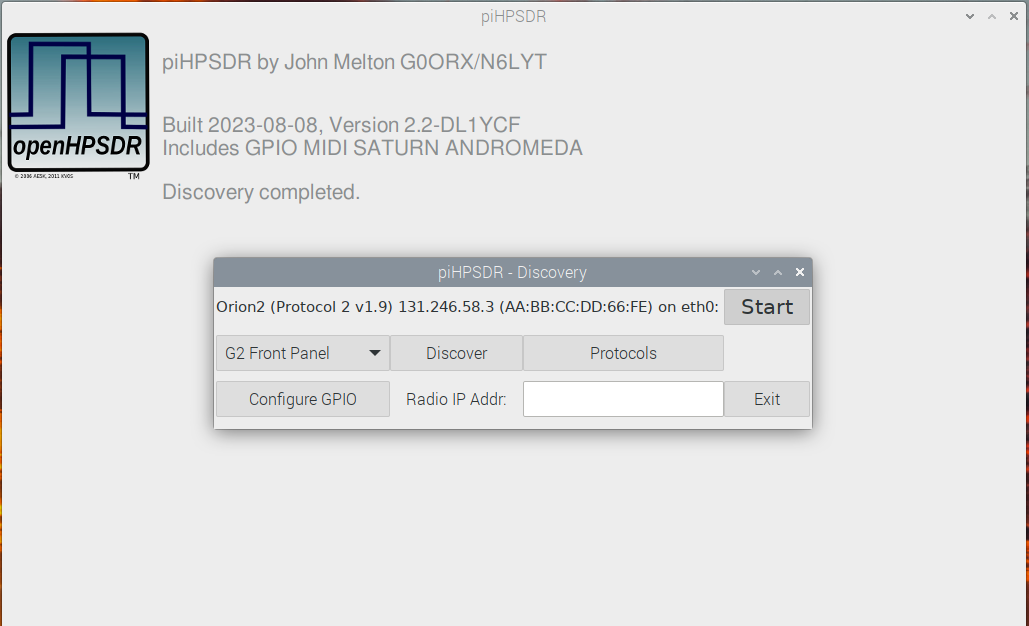
\includegraphics[width=12cm]{Start.png}
\end{center}

At this point, you can start the radio by clicking the \texttt{Start} button, but let us first explain the
purpose of the other buttons! Easiest to explain is the \texttt{Exit} button, this will simply terminate
the program. Most likely, you may want to go into the \texttt{Protocols} menu sooner or later.
 By default, piHPSDR tries to
discover the presence of a radio using all protocols known to piHPSDR. However, if you know that your radio, for
example, uses Protocol 2, then trying to discover a Protocol-1 radio is just a waste of time. So if you
know which types of radio you want to connect to, check these protocols. The available protocols are
\begin{itemize}[font=\texttt, left=80pt]
\item[Protocol 1]{This is the "original" HPSDR protocol.}
\item[Protocol 2]{This is the "new" HPSDR protocol.}
\item[Saturn XDMA]{This is used to talk to a Saturn FPGA through the internal XDMA interface. Only available
if piHPSDR is compiled with the \texttt{SATURN}  option.}
\item[USB OZY]{This is used to talk to a radio using the legacy USB OZY interface. Only available if piHPSDR
is compiled with the \texttt{USBOZY} option.}
\item[SoapySDR]{This is used to talk to a radio through the SoapySDR library, for example to an AdalmPLUTO. 
Only available if piHPSDR is compiled with the \texttt{SOAPYSDR} option.}
\item[STEMlab]{This is used to connect to RedPitaya based SDRs through the WEB interface. Only available if piHPSDR is
compiled with the \texttt{STEMLAB\_DISCOVERY} option. Starting the radio using this protocol is a two-step process:
first, the RedPitaya's WEB interface is located, and the \texttt{Start} button then starts the SDR app
on the RedPitaya. Then, piHPSDR tries to connect to this SDR app and upon success offers a new \texttt{Start} button
to start the radio. If the RedPitaya is exclusively used as a radio, it is recommended to auto-start the SDR app
when the RedPitaya is powered up. In this case, the STEMlab protocol is not used, because the SDR app can be started
through Protocol-2.}
\item[Autostart]{This is a very useful option. It indicates that if exactly one radio has been found, it is automatically
started. So in normal operation, when starting piHPSDR subsequently, and all settings are still valid, the radio is
started without user intervention. If this option is activated and one radio is present, you will not see this menu, so in order
to make further changes here, you have to disconnect the radio from the ethernet cable, start piHPSDR until you see this
menu, and reconnect the radio.}
\end{itemize}

Sometimes piHPSDR needs to know the IP address of the radio. This is, for example, the case for the \texttt{STEMlab} discovery
described above. In such a case the IP address in numerical form (xxx.xxx.xxx.xxx) can be entered in the box
with the label \texttt{Radio IP Addr:}. If a legal IP address is contained in this box, protocol-1 and protocol-2 discoveries
will also send, in addition to a broadcast discovery packet, such a packet to the IP address specified. This way one can
connect to radios which are not on the same subnet as the computer, in principle you can connect to any radio on the world
provided it is on the internet. However, the original HPSDR standard states that a broadcast packet must be used, so several
radios won't reply. On the other hand, there are some radios such as a RedPitaya or a HermesLite-II which allow being discovered
by such a routed packet. 

The \texttt{Discover} button re-starts the discovery process. This is useful if the radio has been powered up too late and
was not yet ready when piHPSDR was started. Simply press \texttt{Discover} to give another try.

The \texttt{Configure GPIO} button opens a menu that currently has no function, so it is not described here.

The combo-box (pop-down menu) to the left of the \texttt{Discover} button lets you choose which type of GPIO controller you
have attached to the computer. This menu is only available if piHPSDR has been compiled with the \texttt{GPIO} option, which
is not the case on desktop/laptop computers. The menu lets you choose between

\begin{itemize}[font=\texttt, left=80pt]
\item[No Controller]{Choose this if no GPIO controller is wired to your Raspberry Pi.}
\item[Contoller1]{Choose this if you have a "version 1" piHPSDR controller.}
\item[Controller2 V1]{This option is valid for some early prototypes of the "version 2" controller.}
\item[Controller2 V2]{Choose this if you have a "version 2" piHPSDR controller.}
\item[G2 Front Panel]{Choose this if you have an ANAN G2 radio with a built-in controller.}
\end{itemize}

\textbf{Attention.} Be sure to choose a controller only if such a controller is actually connected to your Raspberry Pi. If
you choose, for example, a controller which uses an I2C expander for the switches, but no I2C interface is present on
your Raspberry Pi, the program my hang when trying to open the I2C connection.

All settings (protocols, controller, IP address) made in this menu are stored in the global (radio-indepentend) settings
and are restored when piHPSDR is started the next time. 

If all went well, a radio could be discovered and you hit the \texttt{Start} button, you should see the following

\begin{center}
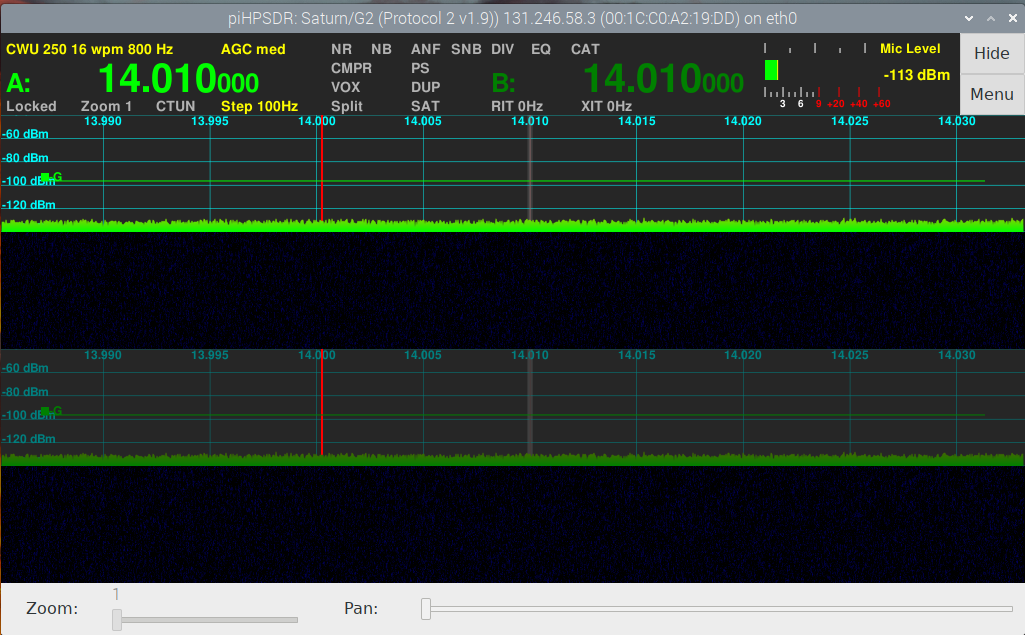
\includegraphics[width=12cm]{FirstDisplay.png}
\end{center}

The bottom of the window looks different (more controls) if you have chosen \texttt{No Controller} in the preceeding menu.
You see two receiver panels stacked vertically, both of them having a spectrum display and a waterfall area. At the top,
just below the window title, you have the VFO bar which contains information on the frequencies of the two VFOs A and B,
as well as lots of further information, to be explained later. At the top right, there are two buttons \texttt{Hide}
and \texttt{Menu} which will be explained in the next chapter. To the left of these two buttons, there is the meter
bar which by default is a digital S-meter. At this point, you have started piHPSDR successfully for the first time.

\chapter{Main window and toolbar}

\begin{center}
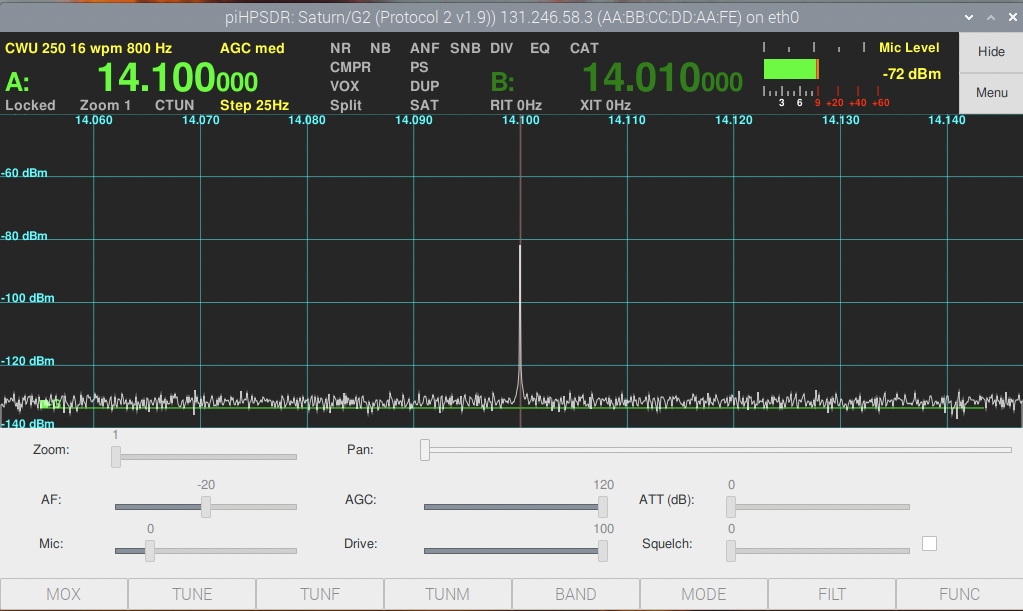
\includegraphics[width=12cm]{SingleReceiver.png}
\end{center}


\begin{center}
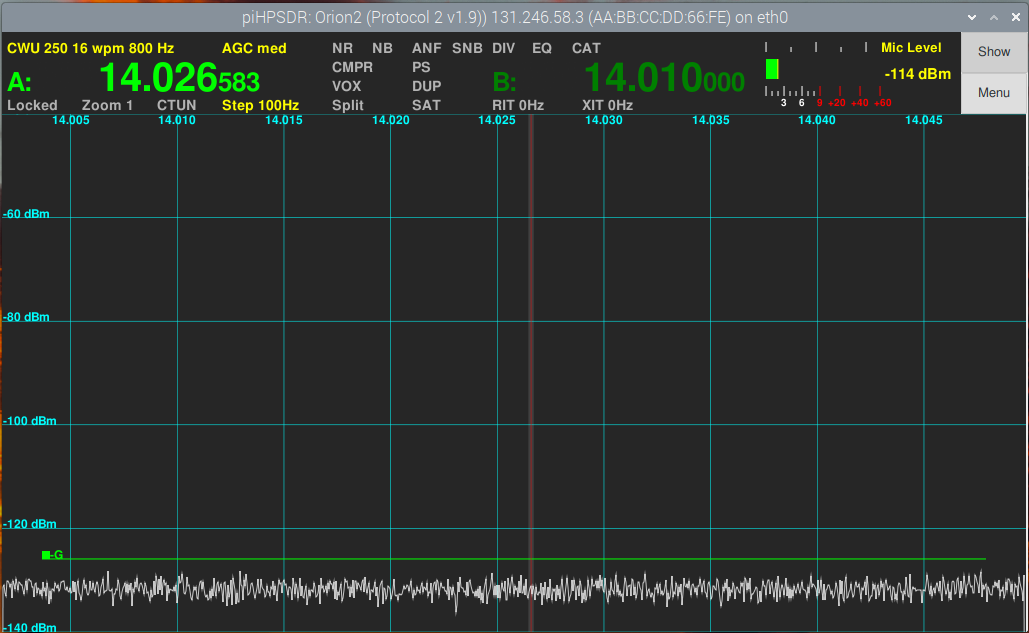
\includegraphics[width=12cm]{Hidden.png}
\end{center}

\section{The VFO menu}
\begin{center}
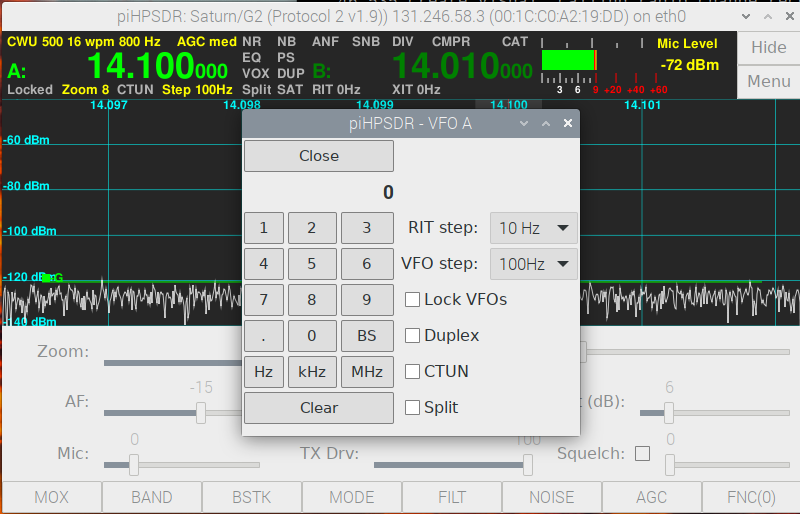
\includegraphics[width=12cm]{VFOmenu.png}
\end{center}

\section{The Meter menu}
\begin{center}
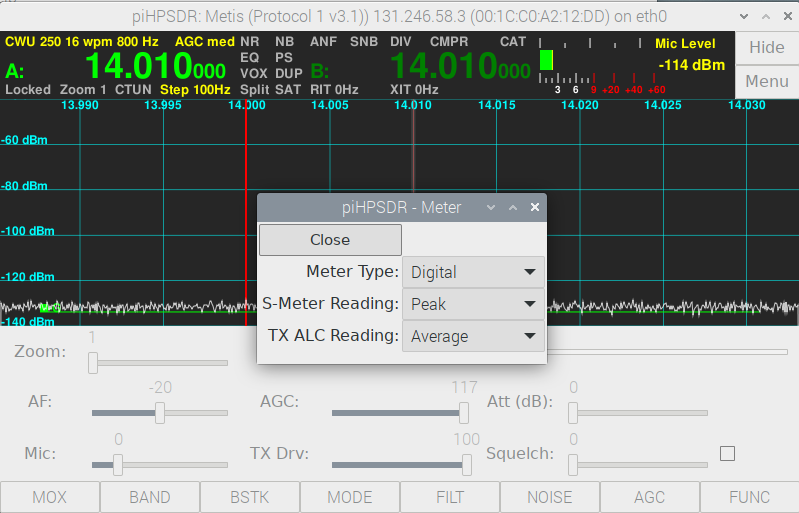
\includegraphics[width=12cm]{MeterMenu.png}
\end{center}

\section{The Band menu}
\begin{center}
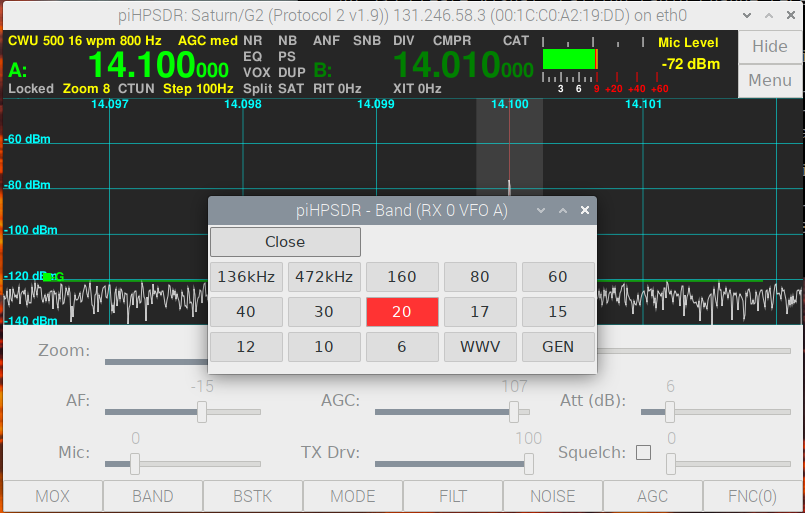
\includegraphics[width=12cm]{BandMenu.png}
\end{center}

\section{The Bandstack menu}
\begin{center}
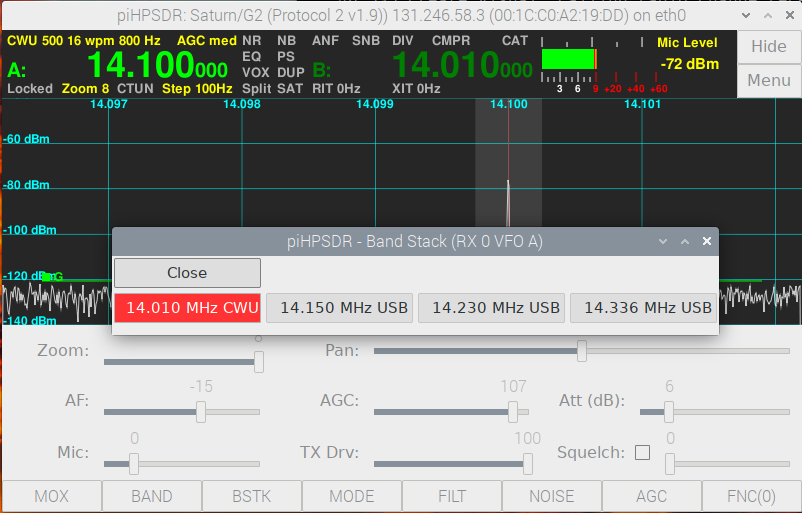
\includegraphics[width=12cm]{BandstackMenu.png}
\end{center}

\section{The Mode menu}
\begin{center}
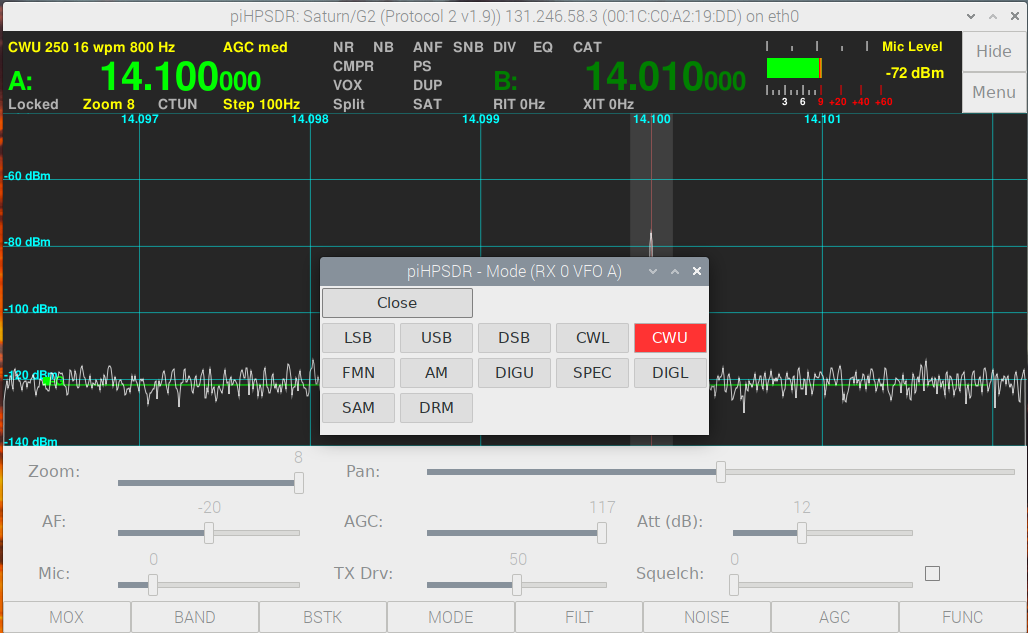
\includegraphics[width=12cm]{ModeMenu.png}
\end{center}

\section{The Filter menu}
\begin{center}
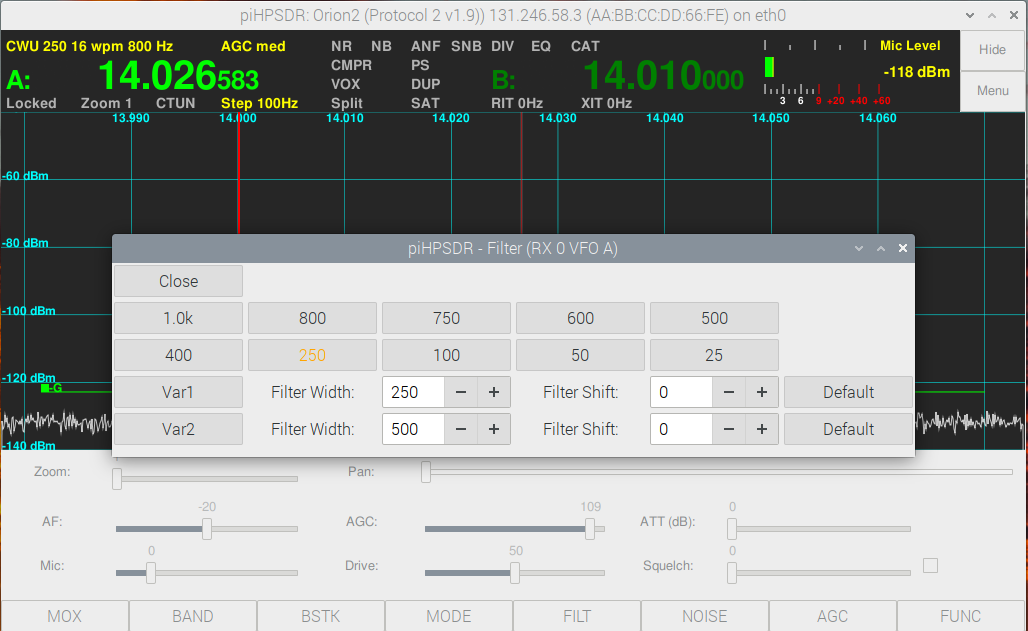
\includegraphics[width=12cm]{FilterMenu.png}
\end{center}

\section{The AGC menu}
\begin{center}
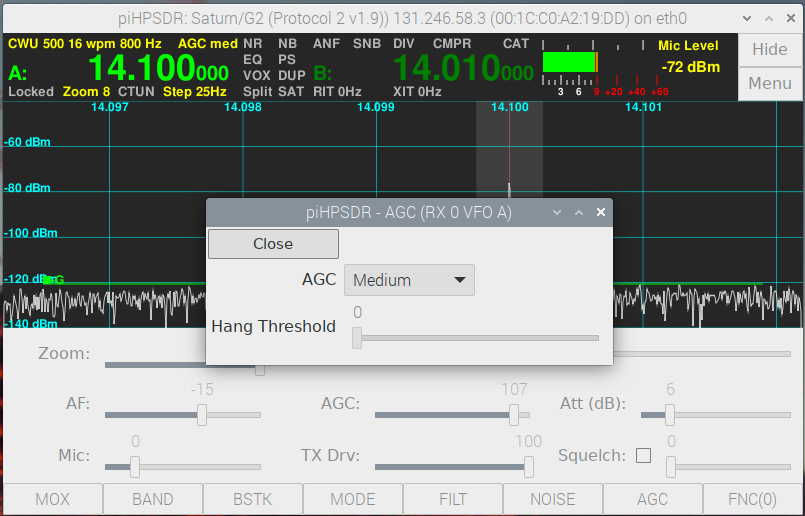
\includegraphics[width=12cm]{AGCmenu.png}
\end{center}

\chapter{The Main Menu: introduction}

\begin{center}
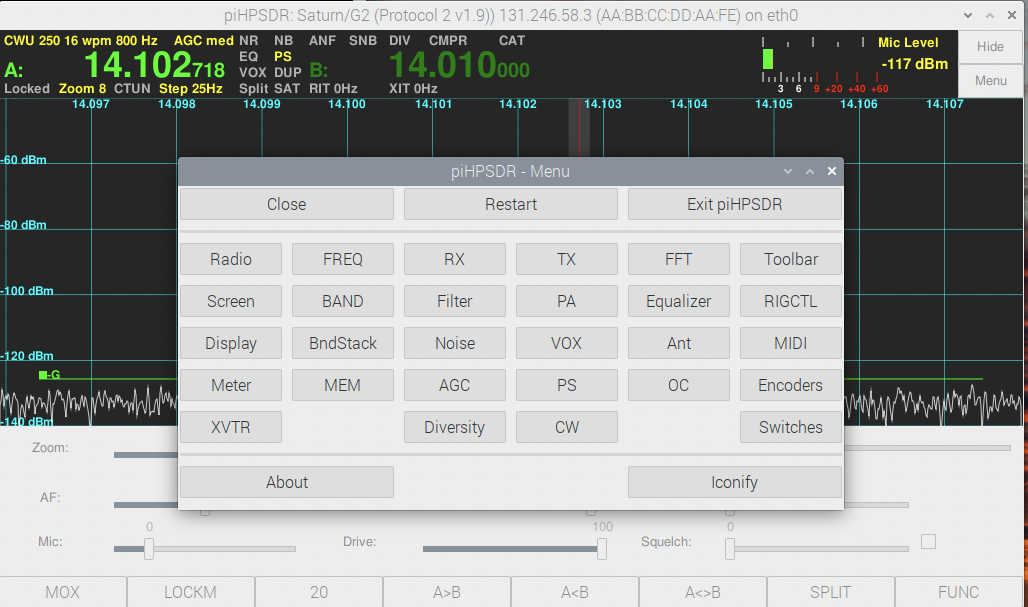
\includegraphics[width=12cm]{MainMenu.png}
\end{center}

\section{The Exit Menu}
\begin{center}
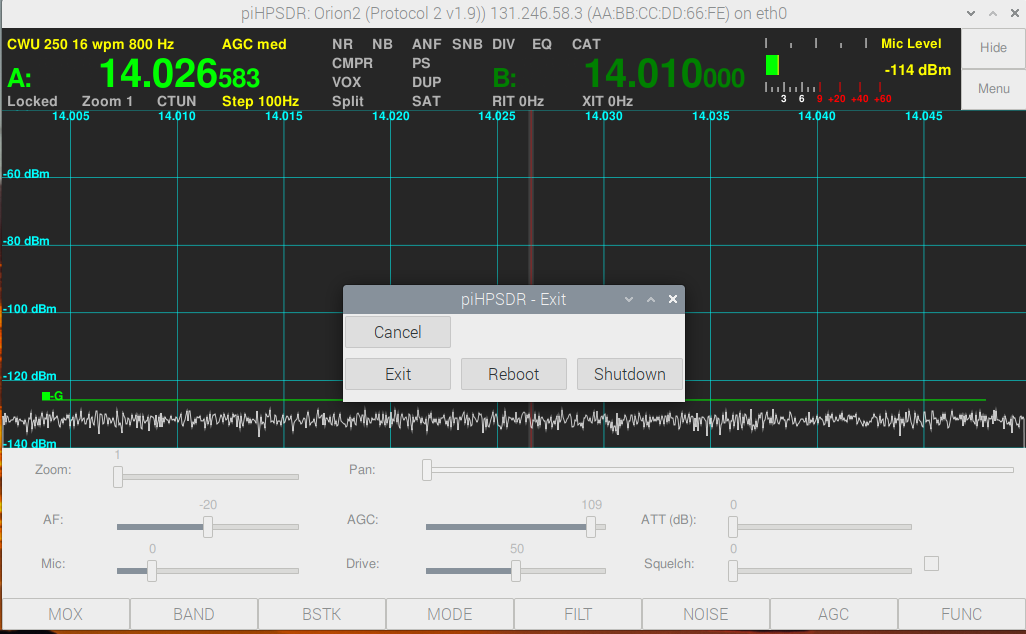
\includegraphics[width=12cm]{ExitMenu.png}
\end{center}

\section{The About Menu}
\begin{center}
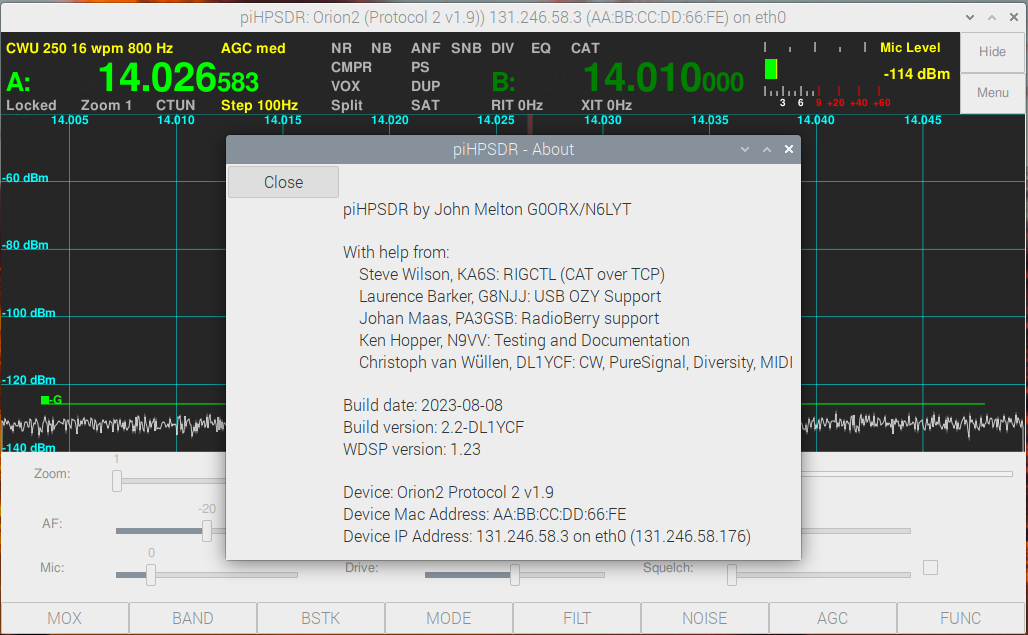
\includegraphics[width=12cm]{AboutMenu.png}
\end{center}

\chapter{The Main Menu: Radio-related menus}

\section{The Radio Menu}
\begin{center}
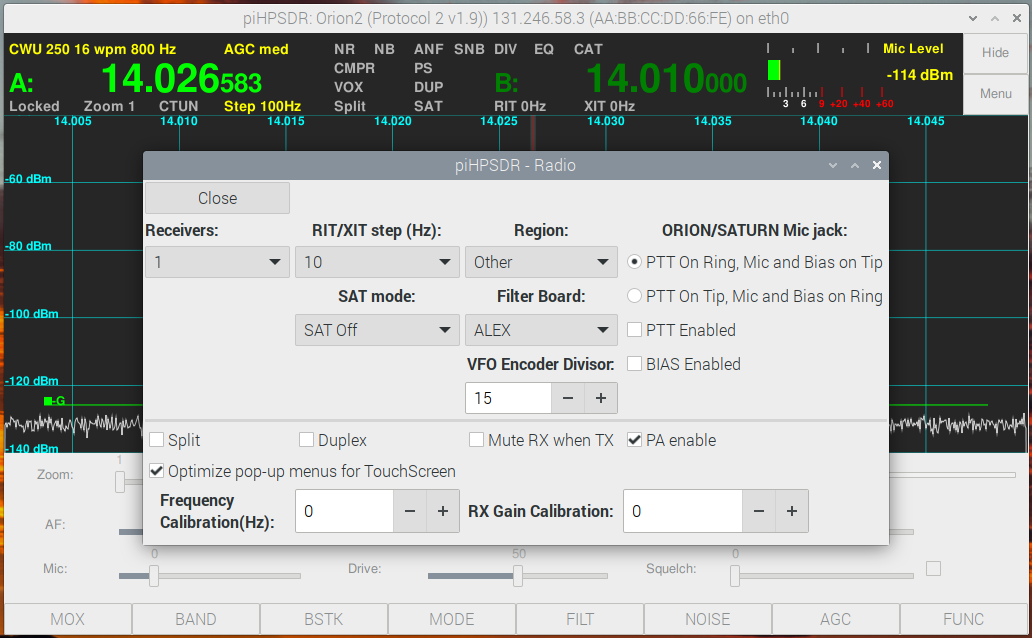
\includegraphics[width=12cm]{RadioMenu.png}
\end{center}

\section{The Screen Menu}
\begin{center}
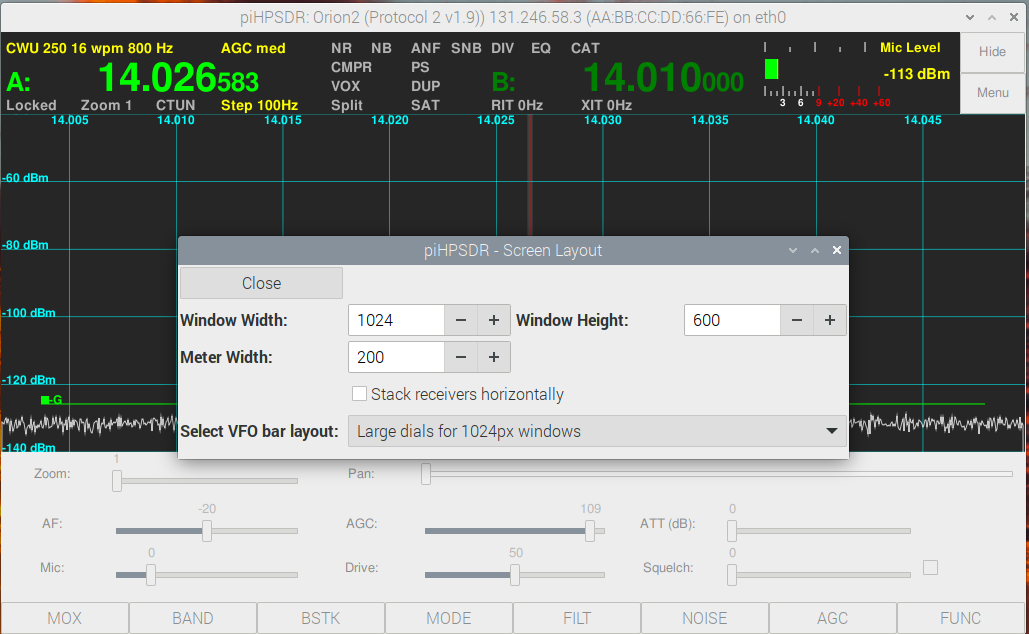
\includegraphics[width=12cm]{ScreenMenu.png}
\end{center}

\section{The Display Menu}
\begin{center}
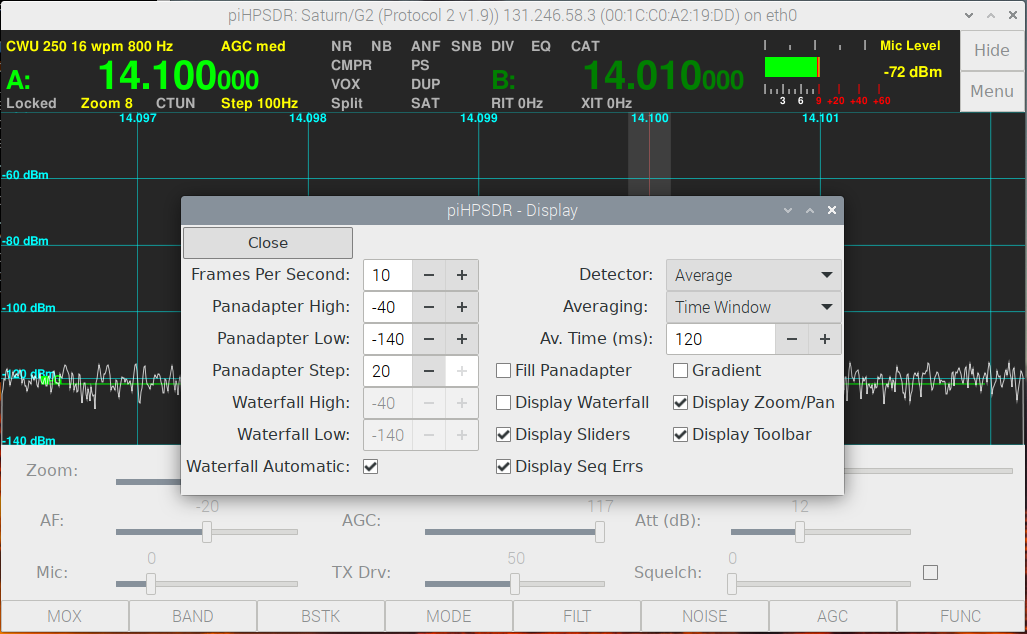
\includegraphics[width=12cm]{DisplayMenu.png}
\end{center}

\section{The XVTR Menu}
\begin{center}
\includegraphics[width=12cm]{XVTRMenu.png}
\end{center}

\chapter{The Main Menu: RX-related menus}

\section{The RX Menu}
\begin{center}
\includegraphics[width=12cm]{RXMenu.png}
\end{center}

\section{The Noise Menu}
\begin{center}
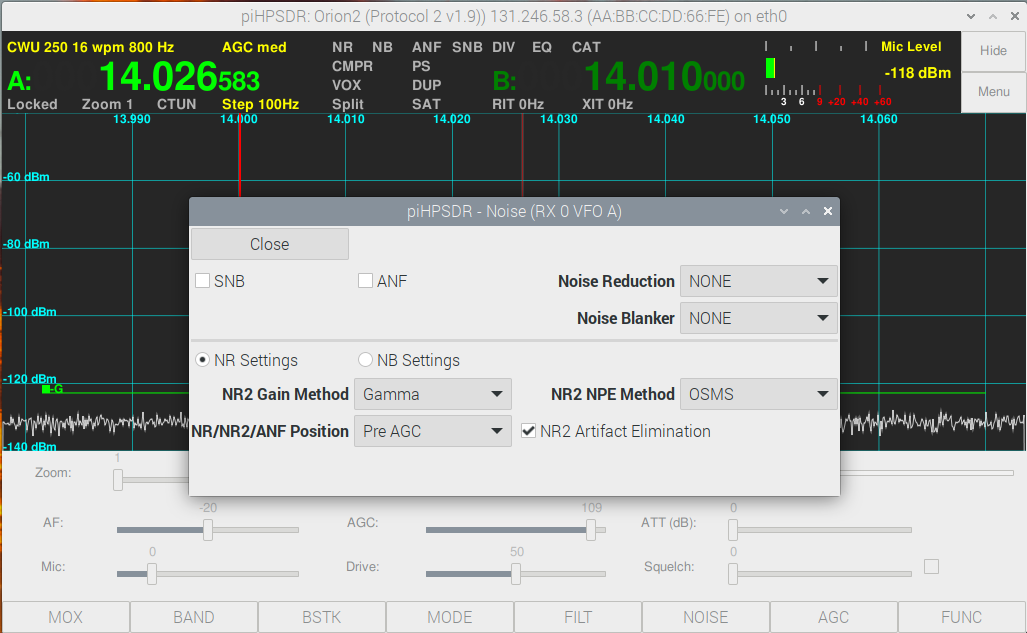
\includegraphics[width=12cm]{NoiseMenu.png}
\end{center}

\section{The AGC Menu}
\begin{center}
\includegraphics[width=12cm]{AGCMenu.png}
\end{center}

\section{The Diversity Menu}
\begin{center}
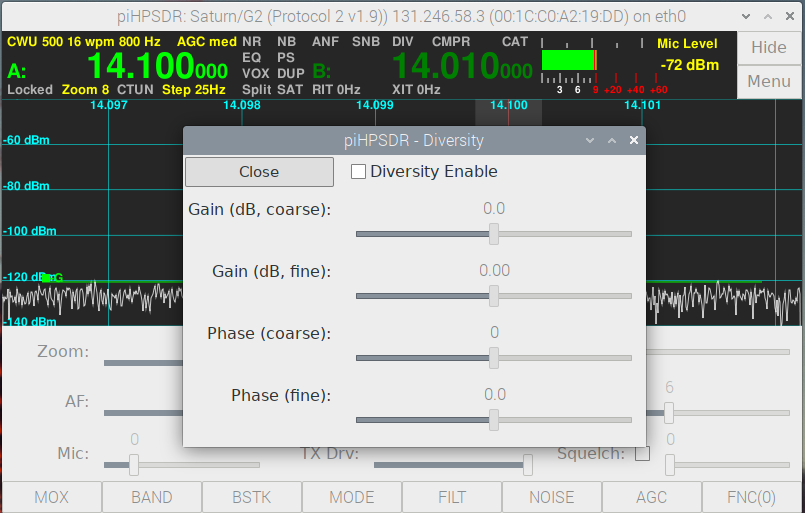
\includegraphics[width=12cm]{DiversityMenu.png}
\end{center}

\chapter{The Main Menu: TX-related menus}

\section{The TX Menu}
\begin{center}
\includegraphics[width=12cm]{TXMenu.png}
\end{center}

\section{The PA Menu}
\begin{center}
\includegraphics[width=12cm]{PAMenuCalibrate.png}
\end{center}

\begin{center}
\includegraphics[width=12cm]{PAMenuWatt.png}
\end{center}

\section{The VOX Menu}
\begin{center}
\includegraphics[width=12cm]{VOXMenu.png}
\end{center}

\section{The PS (PureSignal) Menu}
\begin{center}
\includegraphics[width=12cm]{PSMenu.png}
\end{center}

\section{The CW Menu}
\begin{center}
\includegraphics[width=12cm]{CWMenu.png}
\end{center}

\chapter{The Main Menu: menus for RX and TX}

\section{The FFT Menu}
\begin{center}
\includegraphics[width=12cm]{FFTMenu.png}
\end{center}

\section{The FFT Menu}
\begin{center}
\includegraphics[width=12cm]{FFTMenu.png}
\end{center}

\section{The Equalizer Menu}
\begin{center}
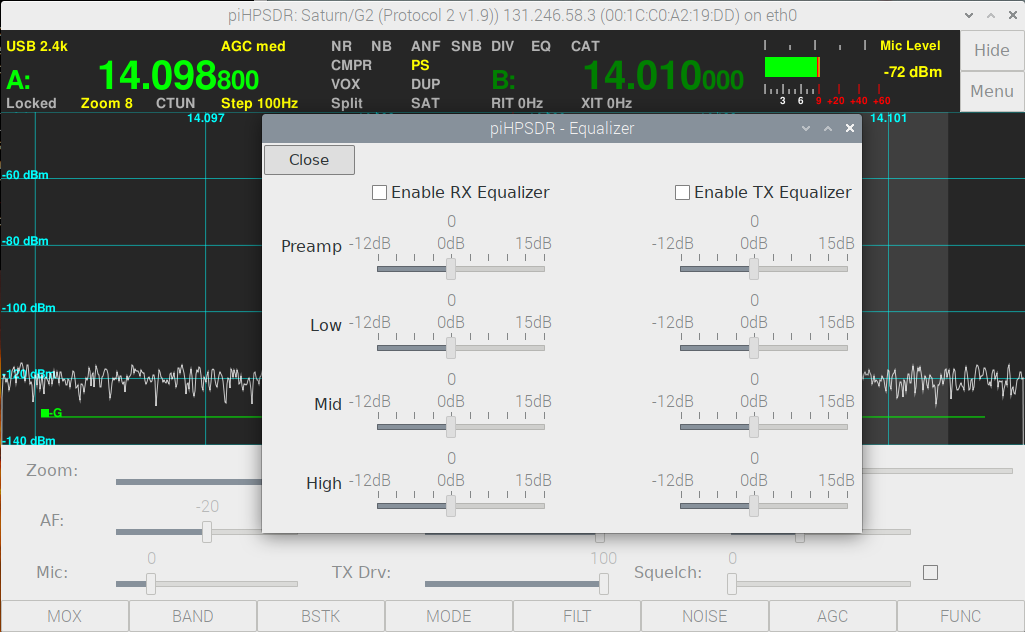
\includegraphics[width=12cm]{EqualizerMenu.png}
\end{center}

\section{The Meter Menu}
\begin{center}
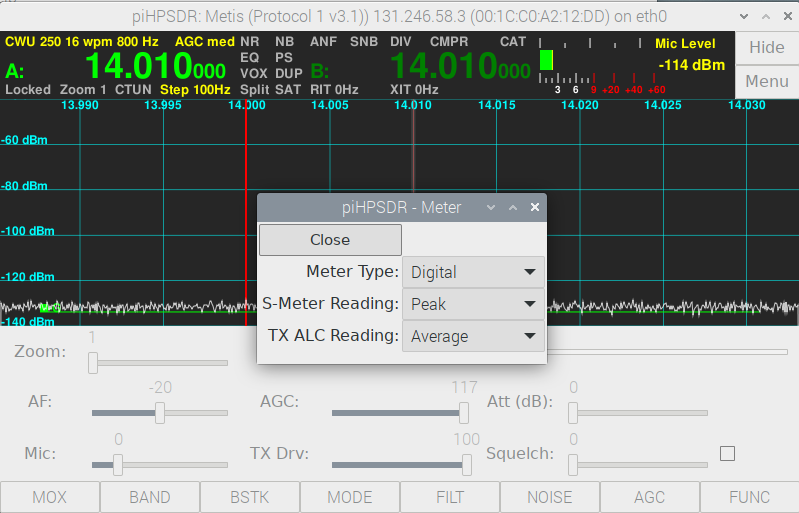
\includegraphics[width=12cm]{MeterMenu.png}
\end{center}

\section{The Ant (Antenna) Menu}
\begin{center}
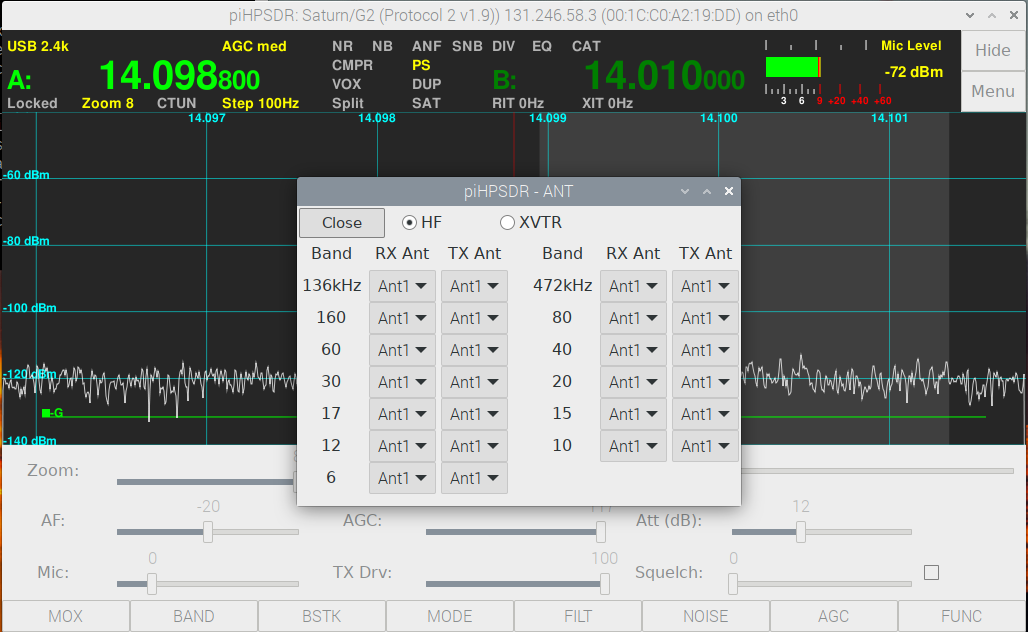
\includegraphics[width=12cm]{AntMenu.png}
\end{center}
 
\section{The OC (OpenCollector) Menu}
\begin{center}
\includegraphics[width=12cm]{OCMenu.png}
\end{center}

\chapter{The Main Menu: controlling piHPSDR}

\section{The Toolbar Menu}
\begin{center}
\includegraphics[width=12cm]{OCMenu.png}
\end{center}

\section{The RIGCTL Menu}
\begin{center}
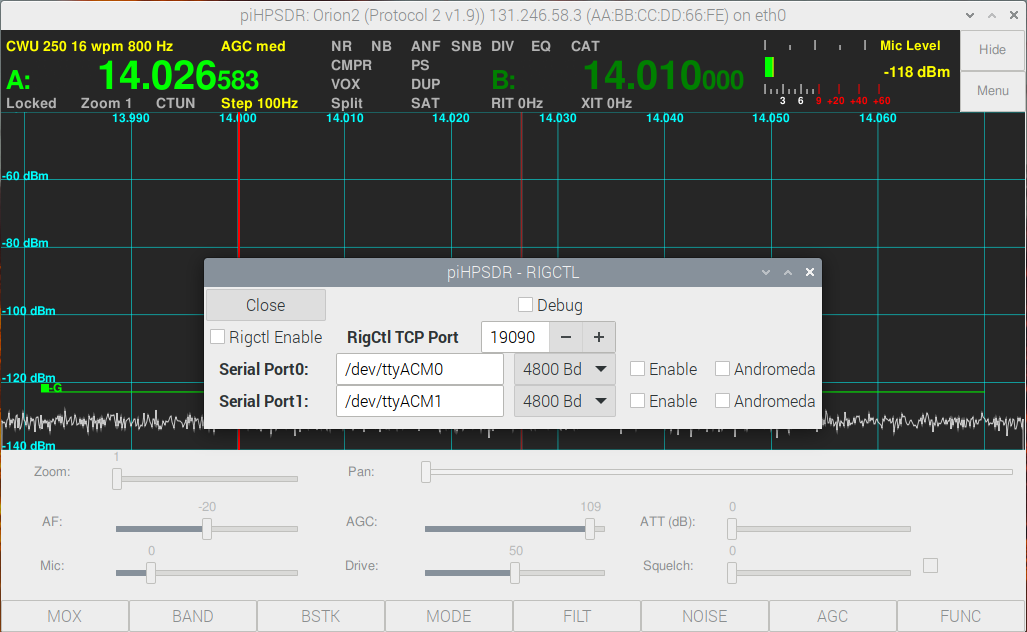
\includegraphics[width=12cm]{RigCtlMenu.png}
\end{center}

\section{The MIDI Menu}
\begin{center}
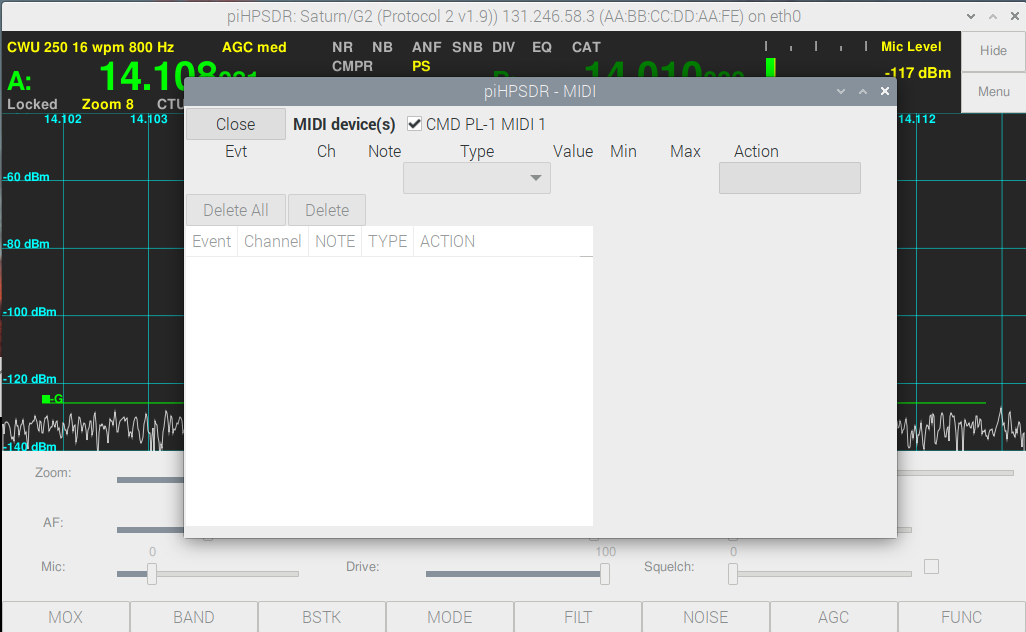
\includegraphics[width=12cm]{MIDImenu1.png}
\end{center}

\begin{center}
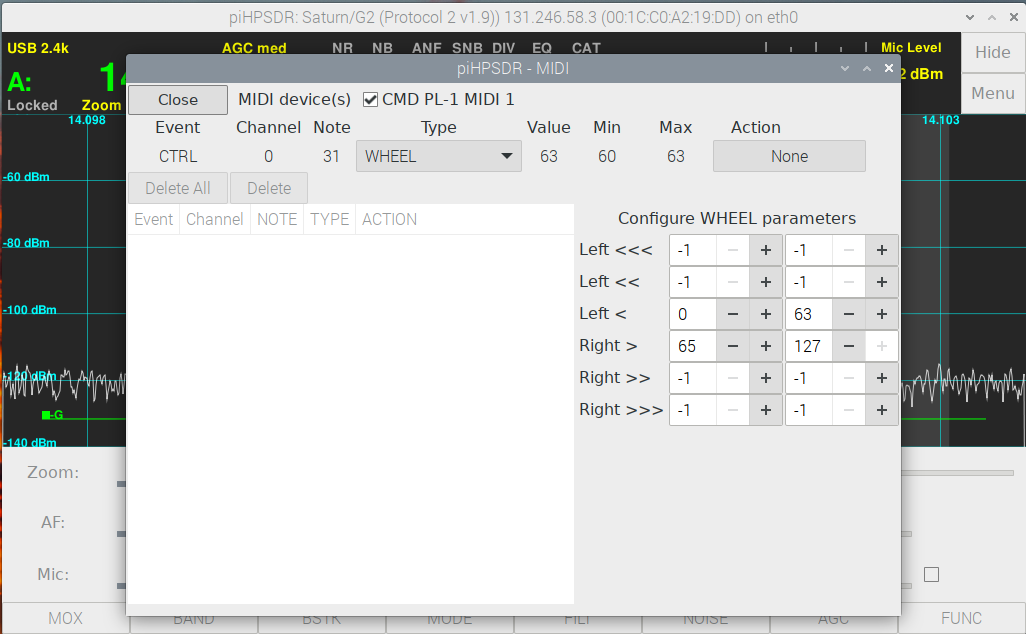
\includegraphics[width=12cm]{MIDImenu2.png}
\end{center}

\begin{center}
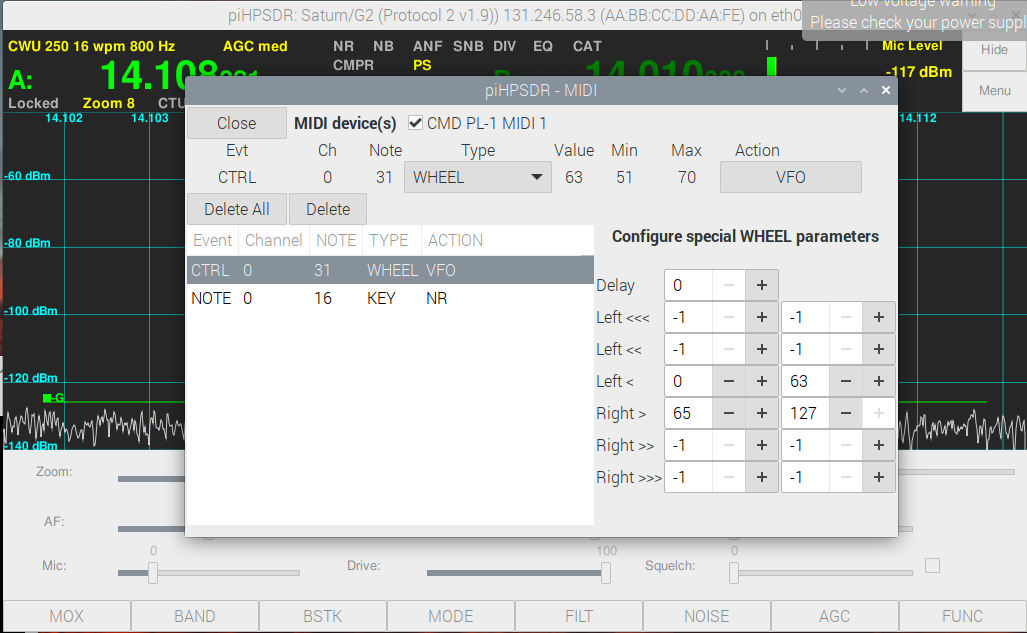
\includegraphics[width=12cm]{MIDImenu3.png}
\end{center}
 
\section{The Encoders Menu}
\begin{center}
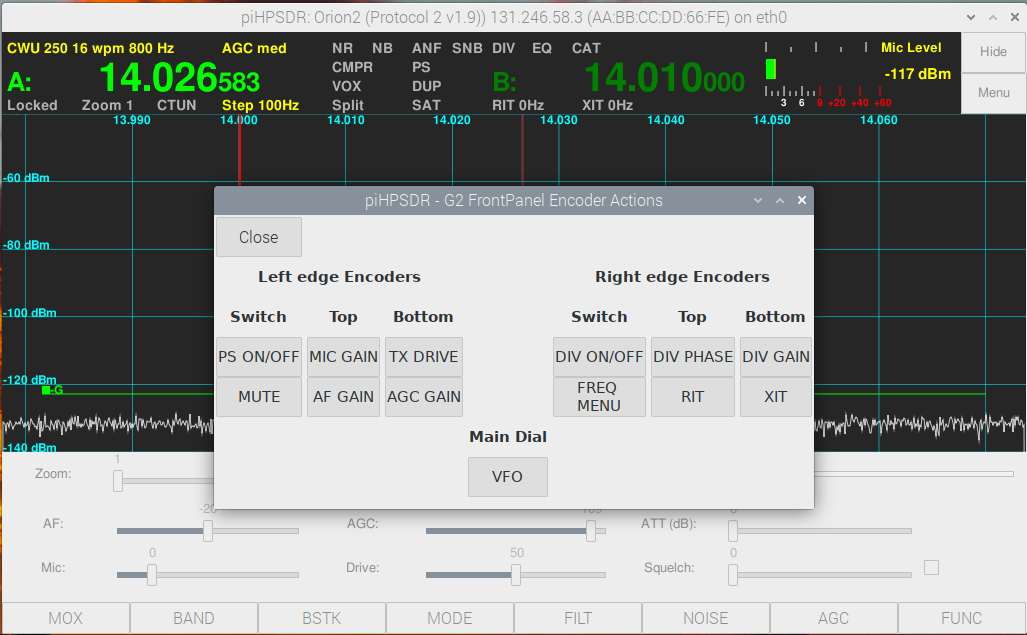
\includegraphics[width=12cm]{EncodersMenu.png}
\end{center}

\section{The Switches Menu}
\begin{center}
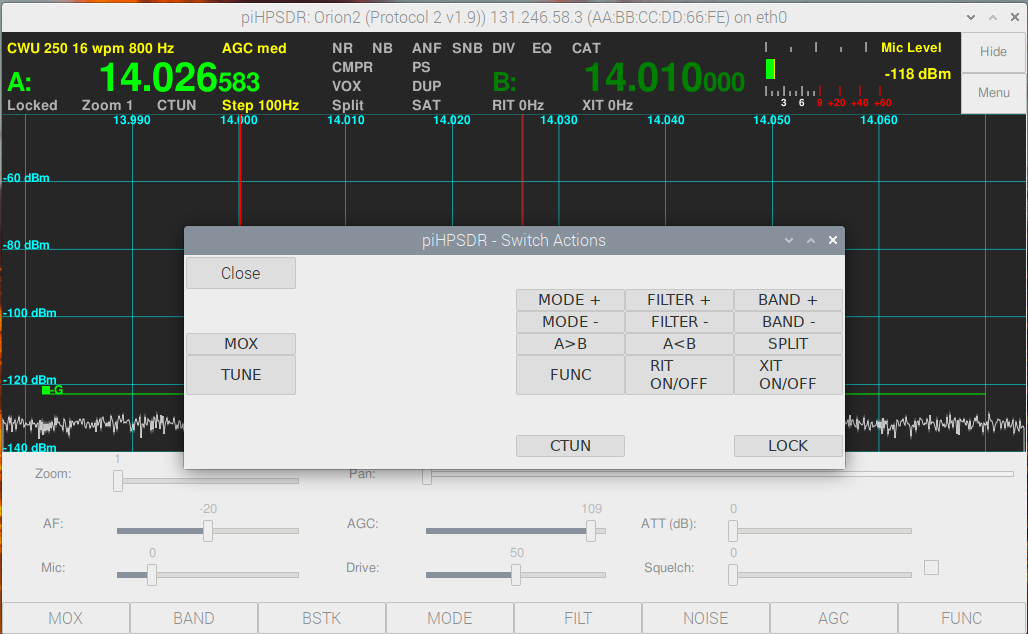
\includegraphics[width=12cm]{SwitchesMenu.png}
\end{center}

\end{document}
